\newpage
\chapter{Literature Review}
\label{Literature}

\lhead{\emph{Literature Review}} % Set the left side page header to "Symbols"



In this chapter we review the theoretical foundations that inform our
computational approach to modeling deliberation. We examine three
interconnected areas: domain restrictions in social choice theory (particularly
single-peaked preferences and hereditary domains), the literature on
deliberation and meta-agreement theory, and computational models of
deliberative processes. Together, these establish both the theoretical
motivation for understanding how deliberation can produce well-structured
preference domains and the methodological foundation for our computational
modeling approach.


\section{Condorcet Domain}
If our goal is to prevent Condorcet cycles, or in general have transitive
majority relations, the best we could hope to do is to apply our domain
restriction such that our domain contains all profiles $\strictProfile$ such that $\strictProfile$ has a
(weak) Condorcet winner. We call this domain $\domain{Condorcet}$. Under this
domain, let $\votingrule{Condorcet}$ be the Condorcet Rule, which picks a
Condorcet winner. Then $\votingrule{Condorcet}$ is strategyproof over
$\domain{Condorcet}$ \citep{elkindPreferenceRestrictionsComputational2022}.

\begin{proofc}{(\citet{elkindPreferenceRestrictionsComputational2022})}.
	Assume, for the sake of a contradiction, we have profiles $\strictProfile = (\pref_1, \dots, \pref_i, \dots, \pref_n)$ and $\strictProfile' = (\pref_1, \dots, \pref_{i'}, \dots, \pref_n)$ such that:
	\[
		\votingrule{Condorcet}(\strictProfile) = a, \quad \votingrule{Condorcet}(\strictProfile') = b, \quad \text{and } a \neq b
	\]
	Assume that $i$ has $b \pref_i a$, thus strictly prefers $b$ to $a$.
	Then under $\strictProfile$ there is a strict majority $C \subseteq N$
	who have $a \pref b$, but $i \notin C$. Thus, in $\strictProfile'$, $C$
	is still a majority preferring $a$ to $b$, making $a$ the Condorcet
	winner in $\strictProfile'$. This is in contradiction to $b$ winning
	in $\strictProfile'$.
\end{proofc}

This result is strengthened by
\citet{campbellNonmonotonicityDoesNot2002,campbellCorrectionStrategyproofnessCharacterization2016},
showing that for an odd number of candidates, \(f_{\text{Condorcet}}\) is the
only voting rule over \(\domain{Condorcet}\) that is strategyproof, surjective
and non-dictatorial.

When surjectivity is strengthened to neutrality, and non-dictatorship to
anonymity, \linebreak \(f_{\text{Condorcet}}\) is the only strategyproof voting
rule over \(\domain{Condorcet}\) for an odd number of voters
\cite{campbellAnonymousNeutralStrategyproof2015}.


Though this result is positive, we might wonder how stable it is. For this we
need to define a notion of stability. On natural way to think about it is as
follows: suppose one of the candidates or voters drops out, do we keep the nice
structure of the domain? If this is true we consider the domain stable and call
it \emph{hereditary}.

\begin{definition}{Hereditary \textnormal{(\citet{elkindPreferenceRestrictionsComputational2022})}}{dom-hereditary}
	A domain $\domain{ }$ is called \emph{hereditary} if for
	every profile $\strictProfile \in \domain{ }$, and every subprofile $\strictProfile'$
	obtained by deleting voters and candidates from $\strictProfile$, it holds that $\strictProfile' \in \domain{ }$.
\end{definition}

$\domain{Condorcet}$ is not hereditary. This is easy to see through an example:

\begin{example}{$\domain{Condorcet}$ is not hereditary}{con-her}
	\begin{minipage}{0.25\linewidth}
		\begin{tabular}{cccc}
			\toprule
			$1$ & $2$ & $3$ & $4$ \\
			\midrule
			$a$ & $b$ & $c$ & $a$ \\
			$b$ & $c$ & $a$ & $c$ \\
			$c$ & $a$ & $b$ & $b$ \\
			\bottomrule
		\end{tabular}
	\end{minipage}
	\begin{minipage}[b]{0.70\linewidth}
		We can see that in this example, $a$ is the weak Condorcet
		winner, as it beats $b$ and is tied with $c$. If we
		remove voter 4 however, we return to the original Condorcet cycle.
	\end{minipage}
\end{example}

If a domain fails to be hereditary, designing an election with the domain is
mind becomes hard. In the case of $\domain{Condorcet}$ it might be reasonable
to make use of a rule such as Black's rule
\cite{blackRationaleGroupDecisionmaking1948}, which uses the Condorcet rule
only if there is a Condorcet winner and the Borda rule otherwise. This however
is not a strategyproof voting rule in general. Instead, we might want to look
at hereditary strategyproof domains. We present the single-peaked domain $\domain{SP}$ , which
will be the main focus of this thesis. This is the domain of all single-peaked
profiles. We first proceed to show that this domain indeed is hereditary.


\begin{proposition}{\textnormal{(\citet{elkindPreferenceRestrictionsComputational2022}).}}
	$\domain{SP}$ is hereditary.
\end{proposition}

\begin{proofc}
	(Voter Deletion). If we remove a voter, this does not affect the other voters, so the profile is still single-peaked.~\checkmark

	(Candidate Deletion). Consider any voter $i$ and their single-peaked
	vote, if we remove some candidate $x$, to this voter all candidates which they preferred to $x$ stay in the same position, while all other candidates move
	up one rank, thus preserving the order, and thus single-peakedness.~\checkmark
\end{proofc}


We have demonstrated that $\domain{SP}$ possesses the desired properties.
However, we currently lack a method to ensure that we operate within
$\domain{SP}$. Deliberation may provide a mechanism to ensure that preference
profiles move toward single-peakedness. We will now provide a concise
overview of the literature on deliberation.

\section{The History of Deliberation and Meta-Agreement}

We have provided an overview of different domain restrictions and their
properties, showing they avoid Condorcet cycles.
\citet{bochslerMarquisCondorcetGoes2010} argues however, that Condorcet cycles
are empirically rare. The next section is dedicated to explaining how
deliberation might explain this is so through examining the historical ideas
around deliberation and deliberative democracy, as well as that of
Meta-Agreement.

\subsection{Deliberation}

Deliberation, though intuitively familiar as
the process of multiple people talking through a problem with the goal of
coming to an agreement, compromise or solution. Providing a definition that is
both clear and consistent with the literature in Political Science, Philosophy
and Social Choice is difficult.  As this intuition leaves some of the reasons for
and goals of deliberation, as stated in the literature, unmentioned.

Instead of defining deliberation in full generality, we instead focus on
deliberation in a political
sense. \citet{freemanDeliberativeDemocracySympathetic2000} gives an overview of
deliberative democracy. He notes that there is no settled definition of
deliberative democracy, however, one account is that of public discussions
before voting. Furthermore, he shares the intuitive idea that a deliberative
democracy contains open legislative deliberation and a pursuit of the common
good. He further proceeds to give a more detailed conception of deliberative
democracy, according to which a deliberative democracy is one in which
political agents or their representatives:

\begin{enumerate}
	\label{list:deliberative-democracy}
	\setlength\itemsep{1px}
	\item  Aim to collect, deliberate and vote
	\item  Represent their sincere and informed judgements
	\item  Vote and deliberate on measures beneficial to the common good for the citizens
	\item  Are seen and see each other as political equals
	\item  Have Constitutional rights and their social means enable them to participate in public life
	\item  Are individually free, such that they have their own freely determined conceptions of the good
	\item  Have diverse and disagreeing conceptions of the good
	\item  Recognize and accept their duty as democratic citizens, and do not engage in public argument on the basis of their particular moral views incompatible with public reason
	\item  Agree reason is public, in so much as it is related to and advances common interests of citizens
	\item  Agree that their common interest lies primarily in freedom, independence and equal status as citizens
\end{enumerate}

These features allow us to be more precise when we talk about a deliberative
democracy, and in turn be more careful about what deliberation must entail.
\citet{cohenDeliberationDemocraticLegimitimacy2002} further argues that
deliberation is needed for democratic legitimacy. By this he means that without
deliberation, a democracy is simply the will of the majority, but since
majority rule is unstable, as shown through the Condorcet cycles, it is simply
a reflection of the particular institutional constrains at the time, which end
up dictating where the cycle breaks. He further goes on to describe the
\emph{ideal deliberative procedure} as follows:

\begin{enumerate}
	\label{list:ideal-deliberation}
	\setlength\itemsep{1px}
	\item  Ideal deliberation is \emph{free}. Participants regard themselves as only bound by the results of the deliberation, and the preconditions thereof. Participants act in accordance with the decision made through deliberation, and it being agreed on is sufficient reason to do so.
	\item  Ideal deliberation is \emph{reasoned}. Participants must
	      state their reasons for supporting proposals.
	\item  In ideal deliberation, parties are \emph{equal}, both formally
	      and substantively. There are no rules that single individuals
	      out, and existing distributions of power to no lend a party the
	      opportunity to contribute to deliberation.
	\item  Ideal deliberation aims to arrive at rationally defensible \emph{consensus}.
\end{enumerate}

From both Cohen's and Freeman's account there is clear overlap, with Freeman
formulating the necessary preconditions for participants to engage in ideal
deliberation. Both Cohen and Freeman  require freedom in a broad sense. Freedom
to have a personal conception of the good, and to acknowledge and act in
accordance to a decision that was made through deliberation.

\subsection{Meta-Agreement}
\label{subsection:Meta-agreement}

Consensus, sometimes referred to as substantive agreement, then seems like a
natural goal for deliberation. \citet{elsterMarketForumThree2002} argues that
this is not only the goal, but through unanimous agreement this process
completely replaces voting, thereby circumventing social choice's classic impossibility
theorems: ``Or rather, there would not be any need for an aggregation mechanism,
since a rational discussion would tend to produce unanimous preferences.'' (p.
112). Though it would be desirable to circumvent these negative results,
in practice people, even after deliberation, might not and indeed often do not
come to full substantive agreement. \citet{listTwoConceptsAgreement2002}
instead proposes another perspective  on deliberation based on Meta-Agreement

Under \emph{Meta-agreement} individuals do not need to agree on their most
preferred outcome, instead they only need to agree on the dimensions of the
problem. To contrast this with Substantive-agreement, under which individuals
do not need to conceive of the problem in the same way, all they need is to
agree on the same outcome. This means that under substantive agreement, voters
can agree outcome $a \pref b$ for different reasons, while under
Meta-Agreement, if voters disagree on $a \pref b$ it must be for the same
reason.

According to \citet{listTwoConceptsAgreement2002} there are three hypotheses that need to be satisfied for deliberation to induce meta-agreement:
\begin{enumerate}
	\label{list:meta-agreement-checklist}
	\setlength\itemsep{1px}
	\item [D1] Deliberation leads people to discover a single \emph{issue}-dimension
	\item [D2] Deliberation lets people place all possible candidates in this \emph{issue}-dimension
	\item [D3] After deliberation, people update their preferences picking
	      a preferred outcome, and ranking all other candidates based on the distance to this outcome in the \emph{issue}-dimension
\end{enumerate}

These are necessary conditions for \emph{meta-agreement}. From this is it also
clear to see that, given that there is exactly one \emph{issue}-dimension,
single-peaked profiles are, by definition, a direct consequence. This property
of inducing single-peakedness makes meta-agreement particularly desirable, as
it enables circumvention of the Gibbard–Satterthwaite theorem
\citep{gibbardManipulationVotingSchemes1973,
	satterthwaiteStrategyproofnessArrowsConditions1975} through
domain restriction to $\domain{SP}$.

\citet{listDeliberationSinglePeakednessPossibility2013} provide empirical
evidence for this theory of deliberation, showing deliberation increases
proximity to single-peakedness through voter deletion (PtS-V), which they define as $S= \frac{m}{n}$
where $n = |\voters|$ and $m$ is the largest subset of voters such that their
profile is single-peaked. Furthermore, they also introduce the notion of
salience, which represents to what extent a topic is salient in the voting
population. In order to test whether deliberation increases single-peakedness
\emph{through} meta-agreement, they test the following four hypotheses: (H1)
deliberation increases PtS-V. (H2')\footnote{This is a
	test for a corollary. H2 states that the rate of increase of PtS-V decreases. This is not experimentally testable, however since
	high salience means some sort of deliberation has happened before, they expect
	this to approximate this affect.} high salience issues show less increase in
PtS than low salience issues. (H3) Effective deliberation, in the sense that
more is learned during deliberation, results in bigger increases of PtS. (H4)
All things equal, the increase is largest for issues with natural
\emph{issue}-dimensions. They find support for all these hypothesis, showing
that on low-moderate salience issues PtS increases following deliberation.

It is important to note that these claims simply predict what will happen,
there is not much explanatory power to these claims. Little is known about to
process be which voters signal the issue dimensions, nor how they decide on
which ones to present.

Furthermore,~\citet{ottonelliElusiveNotionMetaagreement2013} show
single-peakedness from meta-agreement to be a stronger requirement than it may
seem at a first glance. Firstly for (D1) to hold, the \emph{issue}-dimension
must hold some semantic meaning, as it is unclear how people can exchange
conceptualization of the problem otherwise. Furthermore, the issues must
consist of two semantic issues, with only one issue voters simply reach substantive
agreement. A further restriction on these two dimensions is that they need to
be opposite, with opposite justifications. If this is not the case, a voter can
agree with both justifications, and thereby introduce a new implicit dimension
``balance'', which then violates the conditions under which single-peaked
profiles guarantee the existence of fair, strategyproof voting rules. D2
requires that all voters share the exact same semantic understanding of the
dimension, and the outcome associated with each candidate. Finally, D3 requires
D1 and D2 to have happened before in order, indeed this is the weakest of the
three requirements.

Thus, meta-agreement as a means for single-peaked profiles is still quite
restrictive, needing multiple forms of unanimity, and only applying to problems
with certain properties. Nonetheless,  meta-agreement agreement might still
play a crucial part in a deliberative process. In the next section we will
look into a specific computational model of deliberation.


\section{Models of Deliberation} \label{section:related_work} % work on this
\citet{radDeliberationSinglePeakednessCoherent2021} model deliberation
and its effect on single-peakedness. To this end, they model deliberation as
the process of all voters announcing their preferences, and all other voters
updating their current preference towards that of the announced preference, in
doing so they have a bias towards their own preference, as such they try to
update their preference by minimizing the distance between their current
preference and the announced one. This process repeats until all voters have
announced their opinion once, which constitutes one ``round'' of deliberation.
The preference a voter adopts when updating must lie between their current
profile and the announced profile, which profiles are considered to be
``between'' is defined by the distance metric used. They considered three
distance metrics, Kemeny-Snell (KS)~\citep{kemeny1962preference}, Duddy-Piggins
(DP)~\citep{duddyMeasureDistanceJudgment2012}, and Cook-Seiford
(CS)~\citep{cookPriorityRankingConsensus1978}. Both KS and DP depend on the
judgement set resulting from the voters preferences, which is contains, for
each pair of candidates $a,b$, where $a \neq b$, a proposition $(a \pref b)$ or
$\neg (a \pref b)$. The KS distance is then defined as the number of binary
swaps a judgement set needs to undergo before it becomes the target judgement
set, an example for such a swap would be going from $(a \pref b)$ to $\neg (a
	\pref b)$. The DP distance is defined on the graph of judgement sets, where 2
sets share an edge if there is no judgement set between them. Since KS and DP
share their notion of betweenness, we define their betweenness as follows.

\begin{definition}{J-Betweenness}{def:j-between}

	A judgement set $J_i$ is between preferences $J_j$ and $J_k$ if for
	every $x,y \in \alternatives$, the proposition over $x$ and $y$ in
	$J_i$ either agrees with the proposition over $x$ and $y$ in $J_j$ or $J_k$.

\end{definition}

From this definition it is clear that this could only result in a voter
updating their original opinion in which they have $(a \pref b)$ to a new
opinion where $\neg (a\pref b)$ only if the announced opinion contains $\neg (a
	\pref b)$.


The CS distance is simpler and is simply defined as the number of positions two
voters disagree on, and a preference is between two others if for each position
it agrees with one of the two preferences.

Each distance has different trade-offs, CS is the simplest, but might
exaggerate the distance when there are many candidates, for example if two voters
agree on the relative ranking of all but one candidate, which one voter happens
to rank first, thereby shifting the opinion of voter 2 right by one, the CS
distance would conclude that these voters are in full disagreement, while
reasonably one could conclude their opinions do not differ much. The KS
distance, using judgement sets instead of raw profiles, captures this more
effectively, while still being relatively easy to compute, but in case of many
disagreements, it is likely to over count the distance, since the binary
changes do not capture logical necessities. For example, swapping $( a \pref
	b)$ to $\neg (a \pref b)$ must result in $(b \pref a)$ becoming true (in the
case of strict preferences), thus one might reasonably conclude this should
only count as 1 step. DP improves upon this, \Cref{figure:DPDistance} shows a
graph used for the DP distance in the case of 3 candidates. The graph shows the
benefit of using the DP distance, as the edges in graphs automatically include
logical consequences that the KS distance might not account for. In doing
capturing logical consequences, the DP distances becomes much harder to
compute, mainly through the cost of constructing the full graph of judgement
sets, which grows in $f_m = 1 + \sum_{j=1}^{m-1} \binom{m}{j} f_{n-j}$ in the
number of vertices, where $m$ is the number of
candidates~\cite{grossPreferentialArrangements1962}. This can easily be
verified by noting that the number of judgements sets over $m$ corresponds to
the number of weak preference rankings over $m$ candidates, which is defined as
candidates, and a binary choice on each proposition.



\vspace{1em}
\begin{figure}[ht]
	\centering
	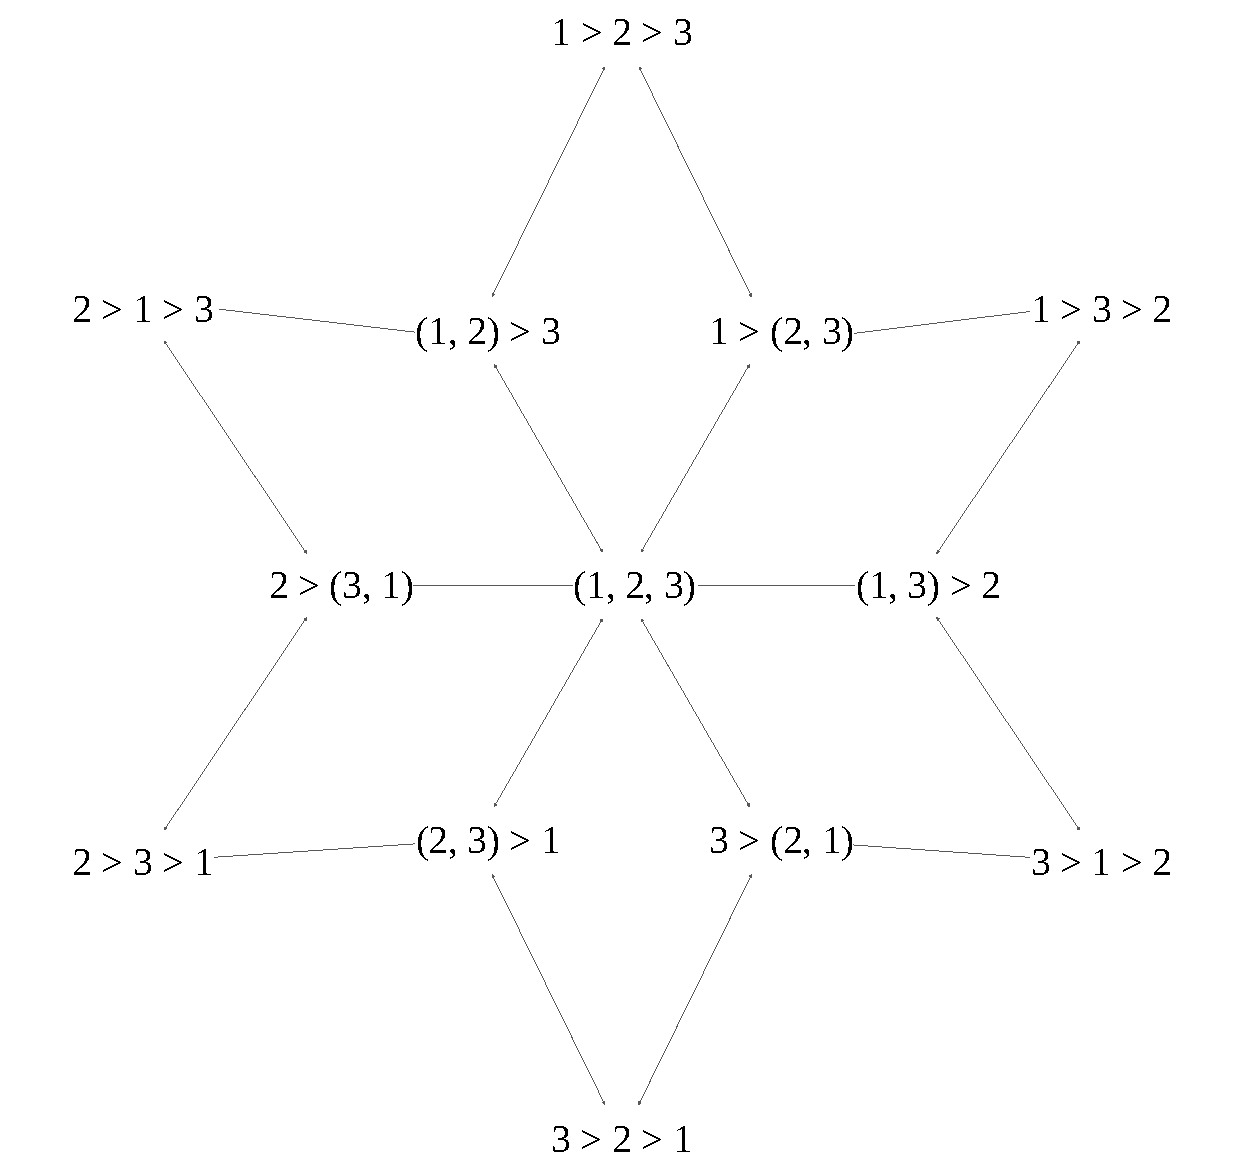
\includegraphics[width=0.65\textwidth]{dpGraph.pdf}
	\caption{The graph of judgement sets for all preferences over three
		candidates, brackets indicate ties. For readability the corresponding
		preferences are uses as node labels}
	\label{figure:DPDistance}
\end{figure}


% TODO D_s should be a map from the set of all possible voters with all
% possible r to the set of all voters TODO also clear up notation, d_s is the
% distance, D_s notation? this is messy

Apart from these distances, Rad and Roy define a voter as a tuple of a linear
order\footnote{We exclude their analysis of preferences containing ties.} and a
bias \(v = \langle r, b \rangle\), with \( b \in \Reals_{[0,1]}\). Finally, a
deliberation step \(D_{s} : V^n \to V^n\), where $V$ is the set of all possible
voters $ (\setOfStrictProfiles \times \Reals_{[0,1]})^n$ and $s$ being one of
the spaces (KS, DP, CS). The deliberation step $D_s(V, v.r)$ returns a fully
updated voter set, where each voter has updated their opinion in response to
the announced opinion $v.r$. We formulate this procedure in the following
program:

\IncMargin{1em}
\begin{algorithm}[H]
	\SetKwInOut{Input}{input}
	\SetKwInOut{Output}{output}

	\Input{Set of Voters $V$, metric space $s$}
	\Output{Updated set of Voters $V$}
	\BlankLine

	$V_{\text{u}} \gets V$ \tcp*[h]{Set of unannounced voters (references to $V$)}\\

	\While{$|V_{\text{u}}| > 0$}{
	Select a random $v \in V_{\text{u}}$\\
	$V_{\text{u}} \gets V_{\text{u}} \setminus \{v\}$\\
	$V \gets D_s(V, v.r)$ \tcp*[h]{Update voters based on $v$'s preference}
	}
\end{algorithm}
\DecMargin{1em}


Here, we use $v.r$ to denote the preference component of voter $v = \langle r, b \rangle$.
The deliberation step $D_s(V, v.r)$ returns a new set of voters, where each voter updates
their opinion based on $v$'s preference $r$, under the influence of the deliberation
space $s$. Each voter updates their preference to a new profile $r'$ that minimizes the weighted distance between their original preference $r_i$ and the announced preference.


\begin{equation}
	\sqrt{
		b d_s(r_i, r')^2 + (1-b)d_s(v.r, r')^2
	}
	\label{eq:deliberation_step_formula}
\end{equation}

Here $b$ is this voter's bias, and $d_s$ is the distance between two profiles
under distance space $s$.

We present a replication and extension of their work \Cref{experiment_results}.
Furthermore, we present novel (negative) results based on this model in
\Cref{theory}.

While this model effectively captures preference communication, it falls short
as a model of meta-agreement in at least two important respects. Firstly,
agents do not conceive of anything relating to the structure of the problem.
They simply announce their preferences, and all other listen and update
accordingly, thereby moving to some sort of substantive agreement. Secondly,
the model presupposes that all opinions are equally defensible, and that each
voter is equally able to formulate this defense. To address this we formulate a
new model in \Cref{theory}.


\section{Deliberative experiments}

We now present some empirical studies showcasing the effects of deliberation in
voting populations, focusing on deliberative policymaking, and the
\textsc{America In One Room} experiment.

\subsection{Deliberative Policymaking}

\subsection{America in One Room}\label{sub:americainonroom} \citet{fishkinCanDeliberationHave2024}
conducted a large scale experiment, during which they brought together American
Voting-eligible citizens to deliberate about policies leading up to the 2020
presidential elections. They conducted a questionnaire on these people
measuring the knowledge of the current state of politics, the opinions on 4
issue domains (Climate, Migration, The Economy, Health Care, Foreign Policy), and
their political affiliation (E.g. Who they would likely vote for, whether they
considered themselves more liberal or conservative). This questionnaire was
also conducted to a control group of people who did not participate in the
deliberation. They found deliberation to increase the likelihood of voting,
improve the opinion on their political rivals, increase the likelihood of
voting for president Biden, among other effects. They explain these effects
through, what they call, ``Civil awakening''. This states that previously
uninformed and uninvolved voters become involved through an increase in
self-efficacy as well as their knowledge. These were still measurable one year
after the intervention. Though they did not measure full preference rankings
over the possible parties, these results do indicate both an increase in
Meta-Agreement, and Substantive-agreement. Namely, in terms of their opinions,
opinions tended to shift more moderate, which more conservative voters changing
their opinions most. The authors also note that moderate voters become more
likely to voter for Biden, indicating some change in how voters conceptualize
of the Candidates' positions.


